\documentclass[tikz,border=2pt]{standalone}
\usepackage{amsmath}
\usepackage{pgfplots}
\pgfplotsset{compat=1.18}
\usetikzlibrary{arrows.meta}
\begin{document}
% Property 1.2(d) for the triangle V with corners (0,0),(4,0),(0,4): x=(1,1) is interior with B(x;0.8) in V, z=(4,0) a corner;
% (1-lambda)x+lambda z=(1+3lambda,1-lambda) has the ball of radius (1-lambda)0.8 in V (radius 0.4 at (2.5,0.5)); the balls shrink to z.
% Tangent points from z to B(x;0.8): (0.947,0.202) and (1.437,1.670).
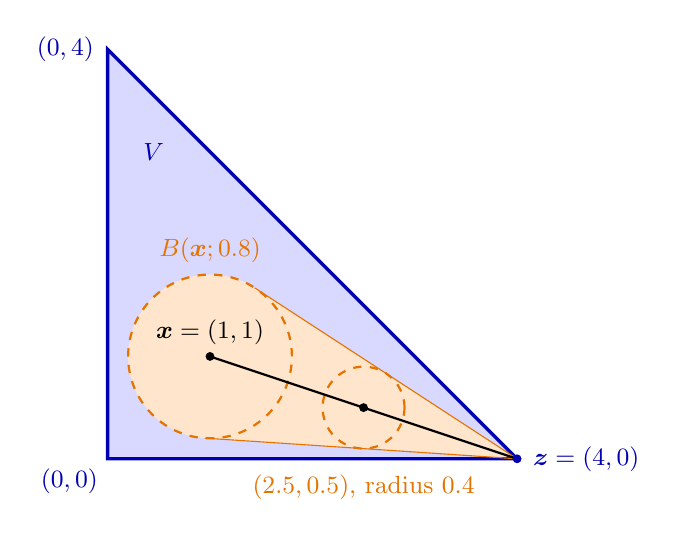
\begin{tikzpicture}[font=\small, >={Latex[length=2mm]}, x=1.3cm, y=1.3cm]
  \fill[blue!15] (0,0) -- (4,0) -- (0,4) -- cycle;
  \fill[orange!20] (4,0) -- (0.947,0.202) -- (1.437,1.670) -- cycle;
  \fill[orange!20] (1,1) circle (0.8);
  \draw[blue!70!black, very thick] (0,0) -- (4,0) -- (0,4) -- cycle;
  \draw[orange!90!black, thin] (4,0) -- (0.947,0.202);
  \draw[orange!90!black, thin] (4,0) -- (1.437,1.670);
  \draw[orange!90!black, thick, dashed] (1,1) circle (0.8);
  \draw[orange!90!black, thick, dashed] (2.5,0.5) circle (0.4);
  \draw[black, thick] (1,1) -- (4,0);
  \fill (1,1) circle (1.6pt);
  \fill (2.5,0.5) circle (1.6pt);
  \fill[blue!70!black] (4,0) circle (1.6pt);
  \node[anchor=south] at (1,1.02) {$\boldsymbol{x}=(1,1)$};
  \node[orange!90!black, anchor=south] at (1,1.82) {$B(\boldsymbol{x};0.8)$};
  \node[blue!70!black, anchor=west] at (4.06,0) {$\boldsymbol{z}=(4,0)$};
  \node[orange!90!black, anchor=north] at (2.5,-0.06) {$(2.5,0.5)$, radius $0.4$};
  \node[blue!70!black, anchor=north east] at (0,0) {$(0,0)$};
  \node[blue!70!black, anchor=east] at (-0.04,4) {$(0,4)$};
  \node[blue!70!black] at (0.45,3) {$V$};
\end{tikzpicture}
\end{document}
